\documentclass[10pt,landscape,twocolumn,a4paper,notitlepage]{article}
\usepackage{hyperref}
\usepackage[english, activeacute]{babel}
\usepackage[utf8]{inputenc}
\usepackage{fancyhdr}
\usepackage{lastpage}
\usepackage{listings}
\usepackage{amssymb}
\usepackage[usenames,dvipsnames]{color}
\usepackage{graphicx}
\usepackage{wrapfig}
\usepackage{amsmath}
\usepackage{makeidx}

%%% Margenes
\setlength{\columnsep}{0.25in}    % default=10pt
\setlength{\columnseprule}{0.5pt}    % default=0pt (no line)

\addtolength{\textheight}{2.35in}
\addtolength{\topmargin}{-0.9in}     % ~ -0.5 del incremento anterior

\addtolength{\textwidth}{1.1in}
\addtolength{\oddsidemargin}{-0.55in} % -0.5 del incremento anterior

\setlength{\headsep}{0.08in}
\setlength{\parskip}{0in}
\setlength{\headheight}{15pt}
\setlength{\parindent}{0mm}

%%% Encabezado y pie de pagina
\pagestyle{fancy}
\fancyhead[LO]{\textbf{\title}}
\fancyhead[C]{\leftmark\ -\ \rightmark}
\fancyhead[RO]{Page \thepage\ of \pageref{LastPage}}
\renewcommand{\headrulewidth}{0.4pt}
\fancyfoot{}
\definecolor{darkblue}{rgb}{0,0,0.4}
%%% Configuracion de Listings
\lstloadlanguages{C++}
\lstnewenvironment{code}
{%\lstset{    numbers=none, frame=lines, basicstyle=\small\ttfamily, }%
	\csname lst@SetFirstLabel\endcsname}
{\csname lst@SaveFirstLabel\endcsname}
\lstset{% general command to set parameter(s)
	language=C++, basicstyle=\small\ttfamily, keywordstyle=\slshape,
	emph=[1]{tipo,usa}, emphstyle={[1]\sffamily\bfseries},
	morekeywords={tint,forn,forsn,fore},
	basewidth={0.47em,0.40em},
	columns=fixed, fontadjust, resetmargins, xrightmargin=5pt, xleftmargin=15pt,
	flexiblecolumns=false, tabsize=2, breaklines, breakatwhitespace=false, extendedchars=true,
	numbers=left, numberstyle=\tiny, stepnumber=1, numbersep=9pt,
	frame=l, framesep=3pt,
	basicstyle=\ttfamily,
	keywordstyle=\color{darkblue}\ttfamily,
	stringstyle=\color{magenta}\ttfamily,
	commentstyle=\color{RedOrange}\ttfamily,
	morecomment=[l][\color{OliveGreen}]{\#}
}

\lstdefinestyle{C++}{
	language=C++, basicstyle=\small\ttfamily, keywordstyle=\slshape,
	emph=[1]{tipo,usa,tipo2}, emphstyle={[1]\sffamily\bfseries},
	morekeywords={tint,forn,forsn,fore},
	basewidth={0.47em,0.40em},
	columns=fixed, fontadjust, resetmargins, xrightmargin=5pt, xleftmargin=15pt,
	flexiblecolumns=false, tabsize=2, breaklines, breakatwhitespace=false, extendedchars=true,
	numbers=left, numberstyle=\tiny, stepnumber=1, numbersep=9pt,
	frame=l, framesep=3pt,
	basicstyle=\ttfamily,
	keywordstyle=\color{darkblue}\ttfamily,
	stringstyle=\color{magenta}\ttfamily,
	commentstyle=\color{RedOrange}\ttfamily,
	morecomment=[l][\color{OliveGreen}]{\#}
}

%%% Macros
\def\nbtitle#1{\begin{Large}\begin{center}\textbf{#1}\end{center}\end{Large}}
\def\nbsection#1{\section{#1}}
\def\nbsubsection#1{\subsection{#1}}
\def\nbcoment#1{\begin{small}\textbf{#1}\end{small}}
\newcommand{\comb}[2]{\left( \begin{array}{c} #1 \\ #2 \end{array}\right)}
\def\complexity#1{\texorpdfstring{$\mathcal{O}(#1)$}{O(#1)}}
\newcommand\cppfile[2][]{
	\lstinputlisting[style=C++]{#2}
}
\begin{document}
	\tableofcontents
	
	\newpage
	
	\section{Template}
	\cppfile{../plantilla.cpp}
	
	\newpage
	
	\section{Data structures}
	
	\subsection{Segment Tree}
	\cppfile{../DataStructures/SexTree.cpp}
	\newpage
	\subsection{Merge Sort Tree}
	\cppfile{../DataStructures/MergeSortTree.cpp}
	\newpage
	\subsection{Fenwick Tree}
	\cppfile{../DataStructures/FenwickTree.cpp}
	\newpage
	\subsection{Sparse Table}
	\cppfile{../DataStructures/SparseTable.cpp}
	\newpage
	\subsection{Disjoint Set Union}
	\cppfile{../DataStructures/DSU.cpp}
	\newpage
	\subsection{Lazy SegTree}
	\subsubsection{Min/Max Range / Single Acces Element}
	\cppfile{../DataStructures/LazyMinMaxSingle.cpp}
	
	% To add
	%	Lazy sum and assigment
	%	Persistent Sextree
	%	Segment Tree multi dim
	%	Wavelet Tree
	%	Treap
	%	Trie
	%	BST
	%	Link cut tree
	%	Monotonic ds
	
	
	
	
	
	\section{Graphs}
	\subsection{DFS}
	\cppfile{../Graphs/dfs.cpp}
	\subsection{BFS}
	\cppfile{../Graphs/bfs.cpp}
	\subsection{Topological Sort}
	\cppfile{../Graphs/topoSort.cpp}
	\subsection{Flood Fill}
	\cppfile{../Graphs/FloodFill.cpp}
	
	
	\subsection{MST}
	\subsubsection{Kruskal}
	\cppfile{../Graphs/Kruskal.cpp}
	
	\newpage
	
	\subsubsection{Prims}
	\cppfile{../Graphs/Prims.cpp}
	
	\subsection{Dijkstra}
	\subsubsection{Implementation}
	\cppfile{../Graphs/Dijkstra.cpp}
	\subsubsection{Space-State graph}
	\cppfile{../Graphs/StateSpace.cpp}
	\subsection{Bellman-Ford}
	\subsubsection{Path}
	\cppfile{../Graphs/BellmanFordPath.cpp}
	\subsubsection{Cycle}
	\cppfile{../Graphs/BellmanFordCycle.cpp}
	
	\subsection{Floyd-Warshall}
	\cppfile{../Graphs/FloydWarshall.cpp}
	
	\subsection{SCC Kosaraju}
	\cppfile{../Graphs/Scc.cpp}
	\subsection{Flows}
	\subsubsection{Dinic}
	\cppfile{../Graphs/Dinics.cpp}
	\subsection{2-SAT}
	\cppfile{../Graphs/2SAT.cpp}
	\subsection{Euler Paths and cycles}
	\subsubsection{Directed Graphs}
	\cppfile{../Graphs/EulerPathsD.cpp}
	\subsubsection{Unirected Graphs}
	\cppfile{../Graphs/EulerPathsND.cpp}
	
	\newpage
	
	\section{Trees}
	\subsection{LCA - Binary Lifting}
	\subsubsection{Normal LCA}
	\cppfile{../Trees/LCA.cpp}
	\subsubsection{Min/Max weight on the path}
	\cppfile{../Trees/MinMaxWeight.cpp}
	\subsection{Centroid Decomposition}
	\cppfile{../Trees/Centroid.cpp}
	\subsection{Euler Tour Technique}
	\cppfile{../Trees/EulerTour.cpp}
	\subsection{Tree Matching}
	\cppfile{../Trees/TreeMatching.cpp}
	\subsection{Diameter}
	\cppfile{../Trees/Diameter.cpp}
	\subsection{Heavy Light Decomposition}
	\cppfile{../Trees/HLD.cpp}	
	
	\section{Math}
	
	\subsection{Identities}
	
	\subsubsection{Combi}
	
	\begin{center}
	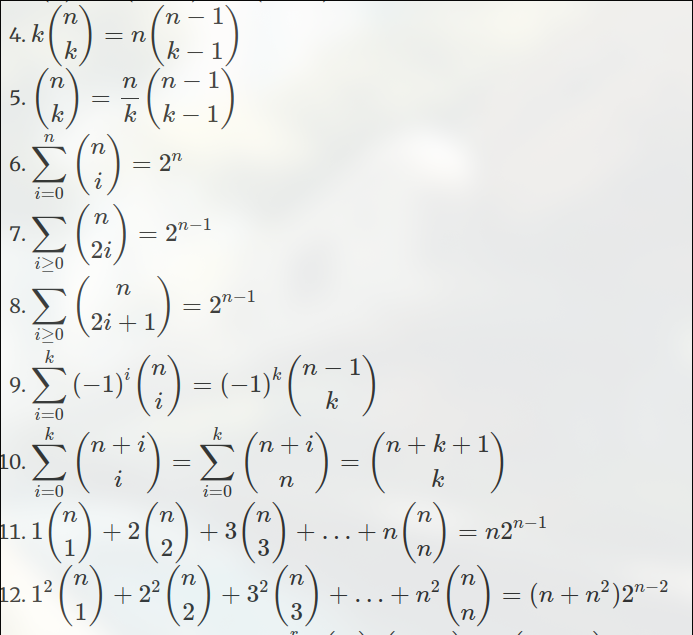
\includegraphics[width=5cm]{Combi2}
	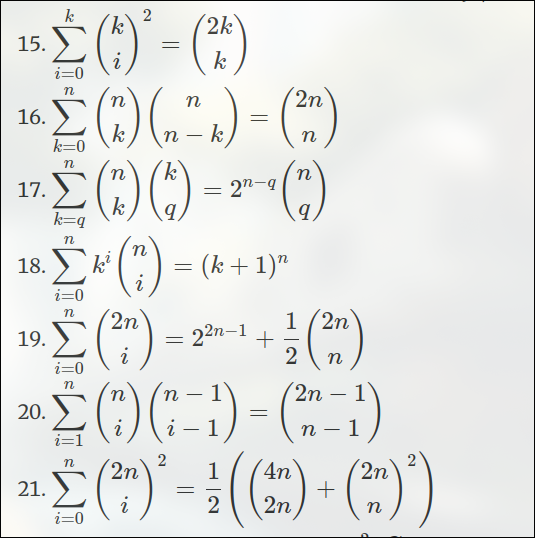
\includegraphics[width=5cm]{Combi}
	\end{center}
	
	\subsubsection{XOR}
	$$ a + b = a \oplus b + 2(a\& b)$$
	$$a + b = a|b + a\&b$$
	$$a \oplus b = a|b - a\&b$$
	$$1\oplus 2\oplus 3 \oplus \dots \oplus(4k-1) = 0  k>=0$$
	
	
	
	
	\subsection{Theorems}
	
	
	\section{Strings}
	\subsection{Suffix Array}
	\cppfile{../Strings/SuffixArray.cpp}
	
	
	
	\section{Others}
	\subsection{Binpow}
	\cppfile{../Others/binpow.cpp}
	\subsection{Matrix exponentiation}
	\cppfile{../Others/MatrixExp.cpp}
	
	
\end{document}